\documentclass[a4paper,12pt,twoside,openright]{book}
\usepackage{bookman}
\usepackage{graphicx}
\usepackage{listings}
\usepackage{fancyhdr} 
\usepackage{color}
\usepackage{ifthen}
\usepackage{epigraph}
\usepackage{url}
\usepackage{rotating}
\usepackage{enumitem}
\usepackage[table,xcdraw]{xcolor}
\usepackage{booktabs,caption,fixltx2e}
\usepackage[flushleft]{threeparttable}
\usepackage[utf8x]{inputenc}
\usepackage{multirow}
\PrerenderUnicode{ăîșțâĂÎÂȘȚ„”}
\setlist[description]{leftmargin=\parindent,labelindent=\parindent}
%\usepackage{showframe}

\usepackage[T1]{fontenc}
\usepackage{inconsolata}

\usepackage{color}

\definecolor{pblue}{rgb}{0.13,0.13,1}
\definecolor{pgreen}{rgb}{0,0.5,0}
\definecolor{pred}{rgb}{0.9,0,0}
\definecolor{pgrey}{rgb}{0.46,0.45,0.48}

\usepackage{listings}
\lstset{language=Java,
  showspaces=false,
  showtabs=false,
  breaklines=true,
  showstringspaces=false,
  breakatwhitespace=true,
  commentstyle=\color{pgreen},
  keywordstyle=\color{pblue},
  stringstyle=\color{pred},
  basicstyle=\ttfamily,
  moredelim=[il][\textcolor{pgrey}]{$$},
  moredelim=[is][\textcolor{pgrey}]{\%\%}{\%\%}
}

\setlength\epigraphwidth{8cm}
\setlength\epigraphrule{0pt}


\newcommand{\newevenside}{
	\ifthenelse{\isodd{\thepage}}{\newpage}{
	\newpage
	\textcolor{white}{placeholder}
	\newpage
	}
}

\newcommand{\code}[1]{\texttt{#1}}

\begin{document}
\thispagestyle{empty}
\begin{titlepage}
	\begin{center}	
		
\includegraphics[width=\textwidth]{../img/header.png}\\[4cm]
		
		{\huge \bfseries \textsc{XCore:\vspace{2.5mm}\\ Support for 
Developing Program\vspace{2.5mm} Analysis Tools}}
		\\[3cm]
		
		{\bfseries Dissertation Thesis} \\[3cm]
								
		\begin{flushright}
				\large Alexandru Ștefănică \\[1cm]
		\end{flushright}
		\begin{flushleft}
			 \large
				\emph{Supervisor} \\
				 Lecturer\\
				Dr. Ing. Petru-Florin Mihancea \\[1cm]
		\end{flushleft}
		
		{\large {Timi\c{s}oara June, 2017}}
	\end{center}
\end{titlepage}

\thispagestyle{empty}
\newevenside

\pagestyle{fancy}
\fancyhead[RE]{\footnotesize{\leftmark}}
\fancyhead[RO]{\footnotesize{\thepage}}
\fancyhead[LO]{\footnotesize{\rightmark}}
\fancyhead[LE]{\footnotesize{\thepage}}
\fancyfoot{}
\setcounter{page}{1}
\tableofcontents

\chapter{Introduction}\label{ch:1}

\epigraph{Any fool can write code that a computer can understand. Good
programmers write code that humans can understand}{Martin Fowler}

\section{Motivation}

        One of the goals of any software developer is to write quality code. Code that respects company policy, that has a
large test coverage percentange, that uses well defined mechanism thus making it portable on different operating system \ldots{} etc. 
In order to establish the quality of encode and enforce different standards analysis tools where build. Some of the most 
used tools are:
        \begin{description}[labelindent=2cm]
        \item[NullTerminator] It represents a pseudo-automatic refactoring tool which 
        eliminates the null checks by use of the \textbf{Null Object Design Pattern} \cite{tools:nullTerminator}
        \item[Wala Tool]  Developed by IBM Research it implements a series of dataflow
        and type analysis algorithms.
        \item[FindBugs]   Widely used tool to detect common programming language hacks
        \item[Intellij IDE] {A platform developed by JetBrains which implements over
        100 code inspector tools}
        \item[CodePro]   A platform which implements software metrics developed by
        LOOSE Research Group. Goes by the name of INCODE, also \cite{tools:inCode}
        \end{description}

        Most analysis tools share a generic back-end which can bee seen in \ref{fig:analysisArchitecture}. The back-end is responseble
for parsing the code in the desired projects and extracting a low-level abstractions / artefacts of the code (e.g the AST of the code). The extracted low-level artefacts,
though usefull, are too granular for most analysis tools, it needs to be processed furthere, resulting in high-level abstractions / artefacts called a \textbf{model}.  This
model is structured according to a \textbf{meta-model} defined and implemented by the developers of the tool. \cite{paper:xcore}

        \begin{figure}
        \centering
        \scalebox{0.3}{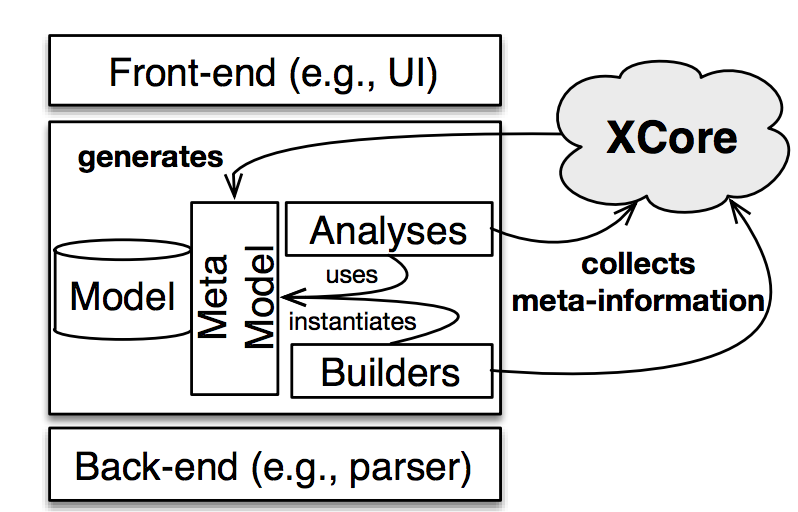
\includegraphics{../img/introduction/analysisArchitecture.png}}
        \caption{Generic Backend for analysis tools \cite{paper:xcore}}
        \label{fig:analysisArchitecture}
        \end{figure}

        The construction of the \textbf{meta-model} is a recuring task when it comes to building analysis tools. \textbf{IPlasma} \cite{tools:iPlasma} uses the \textbf{Memoria}
meta-model in order to compute metrics. Wala \cite{tools:wala} builds its own meta-model in order to preform analysis. Eclipse, as Wala, provides its own meta-model called JDT
\cite{tools:JDT} which is used by most of the Eclipse analysis plugins. 
        
        Building such a meta-model and the necessary back-end is a tedious task, at best. Another major problem that arises when building such a meta-model, and any other program
for that matter, is the evolution in time. We want a meta-mode that can be easily extensible over time, but also have the ability to integrate / inter-operate with other tools / meta-models
in order to obtain complex tools. All of these requirements are difficult to design and implement and, different approaches have been made propoused.\cite{tools:fame} \cite{paper:xcore}
        In order to obtain the mentioned goals, some tools such as inCode\cite{tools:inCode}, have introduced architectural faults which compromised the type safety of the program. This
ultimately lead to poor code which is hard to maintain and understa. \cite{oldThesis}

\section{Previous Work}

        Previously we have build an Ecliplse plugin, called XCore which solved the previously mentioned problems. \cite{oldThesis}. The tool works by providing the software developers with
the means to describe the meta-model of their analysis tool directly into the source code of the tool, without the need to actually implement the meta-model. This is done by providing a higher
level of abstraction called meta-meta-models. The meta-meta-model is implemented by using the java annotations system.\cite{oldThesis} \cite{book:ThinkingInJava} 
        When the tool is compiled, the java compiler will notice the annotations and invoke the XCore annotation process before actually processing the entire project. Our annotation process
will generate, based on the information provided, the appropriate meta-model for the tool and will enforce all the necessary restrictions on meta-model entities. This is perfectly type safe
because after the code generation phase is over the java compiler can fully typecheck the entire system !
        
\section{Current Development}
        
        XCore provides  a way to describe the necessary meta-model for the analysis tool. It also provides a way to integrated a back-end for the extraction of the "meta-model" from the code.
(e.g it can integrate with the eclipse jdt for java meta-mode or eclipse cdt for cpp meta-model). In the previous version you could integrate with only one such back-end, but now we have
modified the implementation such that you can integrate with multiple back-ends. 
        Another major feature that we implemented is that one can extend another analysis tool implemented using XCore.
        Also, we have extended the meta-meta-model description with the concept of Action. One can now describe actions that can be executed upon meta-model entitites. This integrates nicely
with the UI frontend where we could describe an action for opening the analyzed class / method entity in the editor, or concretly pinpoint the design / implementation error in the project.

\section{Related Work}
       
        In essence XCore is a tool for meta-programming. It contains meta-meta-model which allows the user to describe any meta-model respecting the constraints. Thus is bears some similarity
 with other tools which try to solve the problems metioned above, like it such as:
                \begin{description}[labelindent=2cm]
                        \item[Rascal] \cite{tools:rascal}
                        \item[Soot] \cite{tools:soot}
                        \item[Fame] \cite{tools:fame}
                \end{description}
        Rascal is a meta-model programming language. It allows a user to express any meta-model for the development / integration of analysis tools. To the best of my knowledge there is no way
to interact wit other concrete meta-models like those from Wala and Jdt. This is one it's major disadvantage, another being the time and resources need to fully learn the language before using
it. Also, at time of writing, there is also the problem of running time. According to \cite{tools:rascal} the runtime environment is pretty slow.

        Soot is java framework developed for code analysis. It directly analyzes jvm bytecode and can represent in several low level representations. Unlinke XCore, which provides support for 
high analysis tools, the goal of the framework is to provide the necessary tools in order to develope optimization for applications. Also, to the best of my understanding Soot is limited to the
analysis of java byte code, whereas XCore can integrate with and language library backend, provided that the library is written in Java (or C and which can be integrated in Java applications).

        Fame is similar in scope and idea of development with XCore. It uses the FM3 meta-meta-mode \cite{tools:fame} and which is handeled by the JavaFame Tool. The meta-model for the developed
tool is described in a msfe in file. By contract, XCore allows de developers to describe the meta-mode directly in the java source by use of annotations. The main disadvantage in using external
files in order to provide configurations is the lack of support for refactorings (i.e easy change of the meta-model). 




\listoffigures
\listoftables
\bibliographystyle{plain} 
\bibliography{bibliography.bib}

\end{document}
